\section{Decision Trees}
\begin{frame}
   \frametitle{Decision Trees}
   Decision tree inducers provide an algorithm to solve classification and regression problems.
   \begin{itemize}
      \item  A binary decision tree $T$ splits the data: $s_T(x) = x_{i_T} \leq t_{T}$ unless $T$ is a leaf
      \item If $T$ is a leaf, it predicts $T(x) = c_T$ for some constant $c_T$
      \item If $T$ is not a leaf, it creates two subtrees $T_{left}$ and $T_{right}$, and predicts:
      \[   
      T(x) = 
            \begin{cases}

               T_{left}(x) &\quad\text{if}\:  s_T(x) = \text{TRUE} \\
               T_{right}(x) &\quad\text{if}\:  s_T(x) = \text{FALSE} \\
            \end{cases}
      \]
      \item This defines the capacity of the model
   \end{itemize}
\end{frame}


\begin{frame}
   \frametitle{Decision Trees - Example}
   \begin{center}
      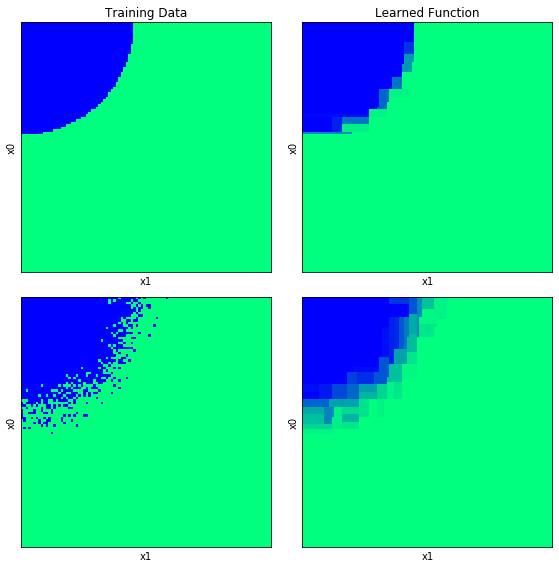
\includegraphics[height=150px]{img/true_vs_learned_regulartree.png}
   \end{center}
   \textit{Left:} Training data of an artificial classification problem. 
   \textit{Right:} Learned function of a decision tree
\end{frame}


\begin{frame}
   \frametitle{Decision Trees - Learning}  
   \begin{itemize}
   \item Fitting a tree is an optimization problem
   \item Many exact solutions are NP hard: e.g. finding a minimal tree that fits the data
   \item Instead of exact solutions: greedy algorithms (bottom up vs top down)
   \item Different loss functions have been proposed: \newline
   InformationGain, Gini Index,  Likelihood-Ratio Chi–Squared Statistics, DKM Criterion, Gain Ratio, ...- see \cite{rokach_decision_2005}
   \item This project evaluates the Information Bottleneck as loss function 
   \end{itemize}
\end{frame}


\begin{frame}
   \frametitle{Decision Trees - Top Down}  
\begin{lstlisting}[language=Python, caption=Python example]
hello
\end{lstlisting}
\end{frame}


% \begin{frame}
%    \frametitle{Decision Trees - Top Down}  
%    \begin{verbatim}
% class DecisionTree():
%   def __init__(self, J, stopping_criterion):
%     self.J = J
%     self.stopping_criterion = stopping_criterion
%     self.p = None

%   def fit(self, X, Y):
%     if self.stopping_criterion(X, Y):
%       self.p = best_constant_estimator(Y)
%       return
%     best_loss = infinity
%     for d in range(X.shape[1]):
%       loss_d, threshhold_d, X_left_d, Y_left_d, X_right_d, Y_right_d = best_split(X[:,d], Y)
%       if loss_d < best_loss:
%         best_loss = loss_d
%         self.threshhold = threshhold
%         self.d = d
%         X_left = X_left_d
%         Y_left = Y_left_d
%       self.left = DecisionTree(self.J, self.stopping_criterion).fit(X_left, Y_left)
%       self.right = DecisionTree(self.J, self.stopping_criterion).fit(X_right, Y_right)
%       return self

%    def predict(self, x):
%      if self.p is not None: \# this tree is a leaf
%        return self.p
%      if x[self.d] < self.theshhold:
%        return self.left.predict(x)
%      else:
%        return self.right.predict(y)

% \end{verbatim}
% \end{frame}